\section{INTRODUCTION}
\label{sec:intro}

%background
Causality plays a critical role in people's daily behaviour and decision-making. Generally, causality is the relation between one event (the cause) and a second event (the effect) in natural language text, where the second event is understood as a consequence of the first event. It is of great interest in many domains, including finance, where understanding causal relationships can provide significant opportunities for economic benefits. Much interesting information appears as natural language text, which must be processed and analysed to derive valuable knowledge. 

%introduce problem
However, exploiting such a kind of causality knowledge is not a easy task, 
the challenges before which are two-fold. Firstly, how to represent causality knowledge, 
Secondly, how to mine causality knowledge from large liberal online text.

%  The rules in this knowledge base can be used to predict financial events and generate alerts in financial trading.
%(TODO: list downstream applications)

\subsection{Challenge 1:Causality knowledge representation.}
%研究背景:别人做得,怎么做得,局限在哪(why you handle this problem)
%
%我们的做法,(how you handle the problem)
%:我们的方法
%:贡献点
%
%举出例子!!


To get some inspirations on how to choose the appropriate causality knowledge representation, we firstly review some related knowledge representation in previous work. 
%%
Now, there are two directions on knowledge representation research. 
The first direction is \textbf{\textit{symbolic form}} for knowledge representation, such as First Order Predicate, \AF{Production, }Semantic Network, Framework. For the way of First Order Predicate, it uses a predicate with several corresponding arguments to represent knowledge. 
%Production is like IF A Then B such kind of knowledge is good at procedural knowledge, which is also based on rule, But such rules need to be elaborated by human. 
Semantic Network represents the knowledge as a network, the nodes of which are abstract concepts like 'bird, 'animal' or concrete nodes like 'canary','dove', and the edges of which are relations like 'kindof', 'ias'. the representative knowledge bases are ConceptNet5 \cite{speer2013conceptnet}, Yago\cite{suchanek2007yago} Freebase\cite{bollacker2008freebase}, and so on. 
Besides, psychological evidence shows knowledge existing in our mind with the form of frames which means frame can also express the knowledge. FrameNet\cite{baker1998berkeley} is such a kind knowledge base where knowledge is describable in terms of information packets called frames. For example, one frame $Commerce\_buy$ from FrameNet contains core frame elements $buyer$ and $goods$, and frame $Getting$ contains core frame elements $recepient$ and $theme$. Different frames can be connected by some relations to represent complex knowledge , the relation between frame $Commerce\_buy$ and frame $Getting$ in Framenet is  $inherits\_from$. All these existing symbolic representation ways are precise in describing knowledge and doing well in reasoning, But they are all lack of causality representation, and also always suffer from the coverage of knowledge or data sparsity. 

\textbf{\textit{Neural form}} is the other direction towards knowledge representation. Such neural numerical knowledge representation is particularly based on distributed representations \citealp{mikolov2013distributed} and neural networks \cite{socher2013reasoning}, \citealp{bordes2013translating}, \cite{bordes2014question}, \cite{bordes2014semantic} \cite{li-16}. Such knowledge representation is very effective to many downstream Natural Language Processing work \cite{hirschberg2015advances}, such as linguistic structure analysis, machine translation, speech recognition, dialogue systems, and so on. such neural numerical approach can well improve the coverage of knowledge, but suffer from the interpretability, and weakness in reasoning.

Above  knowledge representation approaches have kinds of difficulties in  knowledge  representation, and a common disadvantage of these knowledge representation is lack of causality. So We develop a novel and powerful scheme to represent causality knowledge. Here, we will elaborate how the idea comes from step by step.   

%First Order Predicate, Production, Semantic Network are too simple to express the relation, while Framework is the most potential to express the causality knowledge, But which is too coarse, Since the frame elements of the frame if too general to provide useful information. So we propose a scheme trying to depict such causality knowledge.

First of all, causality relation usually contains cause event and effect event. So we firstly try to represent the events. The most simple event representation is structured form likes \textit{(Subject, Predicate, Object)} \cite{ding2015deep}, \cite{ding2016knowledge}, which is also abbreviated as SPO. Also \citeauthor{zhao2017constructing} just use verbs and nouns to represent the event since the data they use is short news headlines which is hard to extract the complete SPO structure for each headline. Here we would like to adopt the structured form to represent the events like SPO. However informative causality event would give better understanding of the causality, so we expand the SPO form to \textit{(Compound Nouns Of Subj, Subj, Predicate, Compound Nouns Of Obj, Obj)} form which is abbreviated as NSPNO. NSPNO can capture more rich event information than SPO, meanwhile it can be degenerate to the SPO automatically, which means it is compatible with SPO. Event representation is the first key component of causality knowledge representation scheme, which is flexible by substituted it with other event representation scheme, such as NestIE \citeauthor{bhutani2016nested}.

After developing the event representation scheme, hopefully, we wish extract the specific causal event pair from liberate text like \textit{(Compound Noun Of Subj, Subj, Predicate, Compound Noun Of Obj, Obj) $->$ (Compound Noun Of Subj, Subj, Predicate, Compound Noun Of Obj, Obj)}, which is abbreviated as
\begin{equation} 
(NS_c, S_c, P_c, NO_c, O_c)->(NS_e, S_e, P_e, NO_e, O_e)
\label{notation:rule_instance}
\end{equation}
, and we call it \textit{rule instance}. But the cause event and effect event in the rule instance are to specific, so we need to generalize it with a general form to represent a similar class of events. Inevitably, we would conceptualize some of the arguments(subject, object or the component nouns and so on) in the rule instance. Then, we can get the generalized rule instances as following, we call it candidate rule. argument conceptualization is the second key component of our causality knowledge representation scheme. This component makes our causality knowledge representation hierarchical, since we can generalize the rule instances into different concept granularities distributed in different candidate rules. with conceptualization, We can also alleviate the low coverage problem existed in specific rule instances, since concept itself represent lots of arguments in one class, so deriving one candidate means gaining lots of rule instances.  

\begin{equation}
\begin{split}
&(X_0, S_c, P_c, NO_c, O_c)->('', X_1, P_e, NO_e, O_e)\\
&X_0 \ \ IsA \ \ C_1, C_2\\
&X_1 \ \ IsA \ \ C_3
\end{split}
\label{notation:candidate_rule}
\end{equation}

Here is a specific example, one rule instance \ref{notation:rule_instance} would be 
\begin{equation} 
\begin{split}
&\text{('乙醇', '消费量', '增加\_1', '', '')} -> \text{('玉米', '需求量',}\\
& \text{'升高\_1', '', '')}
\end{split}
\label{notation:rule_instance_example}
\end{equation}
After intermediate processes, we get candidate rule (\ref{notation:candidate_rule}) like

\begin{equation}
\begin{split}
&\text{('X0','消费量', '增加\_1', '', '')}-> \text{('X1', '需求量',}\\
&\text{'升高\_1', '', '')} \\
&'X0':\text{['有机溶剂','生物燃料']}\\
&'X1':\text{['作物','谷类']}
\end{split}
\label{notation:candidate_rule_example}
\end{equation}

After generalizing from rule instance, we find the generalized candidate rule is too general, even wrong. For example, we instantiate the candidate rule with $X_0$ to '乙醇' and $X_1$ to '燕麦'. This instantiation satisfies the candidate rule's requirement, but it is unreasonable since '燕麦' is seldom used to produce '乙醇'. So the generalized candidate rules further need some constraints. Here, we add some relations between arguments to candidate rule, then the candidate rules with relation constraints would be real rules. The relation constraints of (\ref{notation:candidate_rule_example}) should be $X0 \ madeof \ X1$. After adding the relation constraint, we will exclude the case of $X_0$ is '乙醇' and $X_1$ is '燕麦', since they don't satisfy the 'madeof' relation constraint. Relation constraint is the third key component of out causality knowledge scheme. So we finally formalize the causality knowledge , which is also called rule, with the following form:

\begin{equation}
\begin{split}
&(X_0, S_c, P_c, NO_c, O_c)->('', X_1, P_e, NO_e, O_e)\\
&X_0 \ \ IsA \ \ C_1,\ C_2\\
&X_1 \ \ IsA \ \ C_3\\
&X0 \ \ relation \ \ X1 
\end{split}
\label{equ:rule_notation}
\end{equation}

Up to now, We elaborate all the procedure of how we represent the causality knowledge, generally from rule instance, to candidate rule ,last to rule.
 
\TD{We need notice such relation is not found by chance. It is in fact because that one event cause another event, Some connection must exist these two events,which is the Do-theory in causality test theory.TODO(give more explanation and citation)} 

\textbf{Contributions.}
The advantages of above causality knowledge representation scheme can be summarized as following:
\begin{enumerate}
	\item \textbf{Natural ability to reason.} Causality is particularly for reasoning
	\item \textbf{Interpretable.} Symbolic form makes it interpretable
	\item \textbf{Hierarchical} our rules are conceptualized with different concept granularities.
	\item \textbf{High coverage} our rules with conceptualization can be instantiated into lots of rule instances, which highly improve the coverage of rule instances.
	\item \textbf{Scalable.} The first key component of our causality knowledge representation can be substituted by other event representation scheme.
	\item \textbf{Portability to Prolog \footnote{ \url{ https://en.wikipedia.org/wiki/Prolog }}.} our causality knowledge representation is very easy used in Prolog.
\end{enumerate} 

In this part, we develop a scheme to represent causality knowledge,
such symbolic causality knowledge representation is interpretable, hierarchical, scalable, and has the ability to reason, portability to Prolog and has high coverage to causality knowledge.

\subsection{Challenge 2: Causality knowledge mining.}
%研究背景:别人做得,怎么做得,局限在哪(why you handle this problem)
%
%rule instance 
%
%我们的做法,(how you handle the problem)
%:我们的方法
%		:the generalization from rule instances to rules mainly has two parts, one is finding Concept Constraint of Arguments and the other is finding Relation Constraint Between Arguments, and We need to exploit external knowledge base. 
%		解释一下为什么需要这两个步骤,也就是为什么要构建knowledge base,在approach中就可以直接引用了 
%		
%		解释为什么要commonsense relation.  这里最好给一个hypothesis 
%		Finding Relation Constraint Between entities if a effective way to specialize the rule after generalize the rule. After watch much examples, We find most the relation between two entities in cause and effect can be connected using commonsense. we can often see corn and alcohol, rubber and oil occured in causal event pairs. emiting  the commnosense relation gap from cause to effect do not affect people's mind, But If we wan't to capture the general rule behind the rule instance, We need dig it out. We inevitably need a large commonsense base. So we build a new commonsense based on ConceptNet5, Probase, WebBrain, WebChild.   
%:贡献点

After developing the scheme for causality knowledge representation, we need to tackle how to discover causality knowledge from large liberal text. Figure \ref{fig:overview} sketches our proposed framework about how to derive the causality knowledge. It is mainly composed by four key components: rule instance extraction, constructing a knowledge base, rule generalization, rule specialization. 
 \begin{figure*}[htbp]
	\centerline{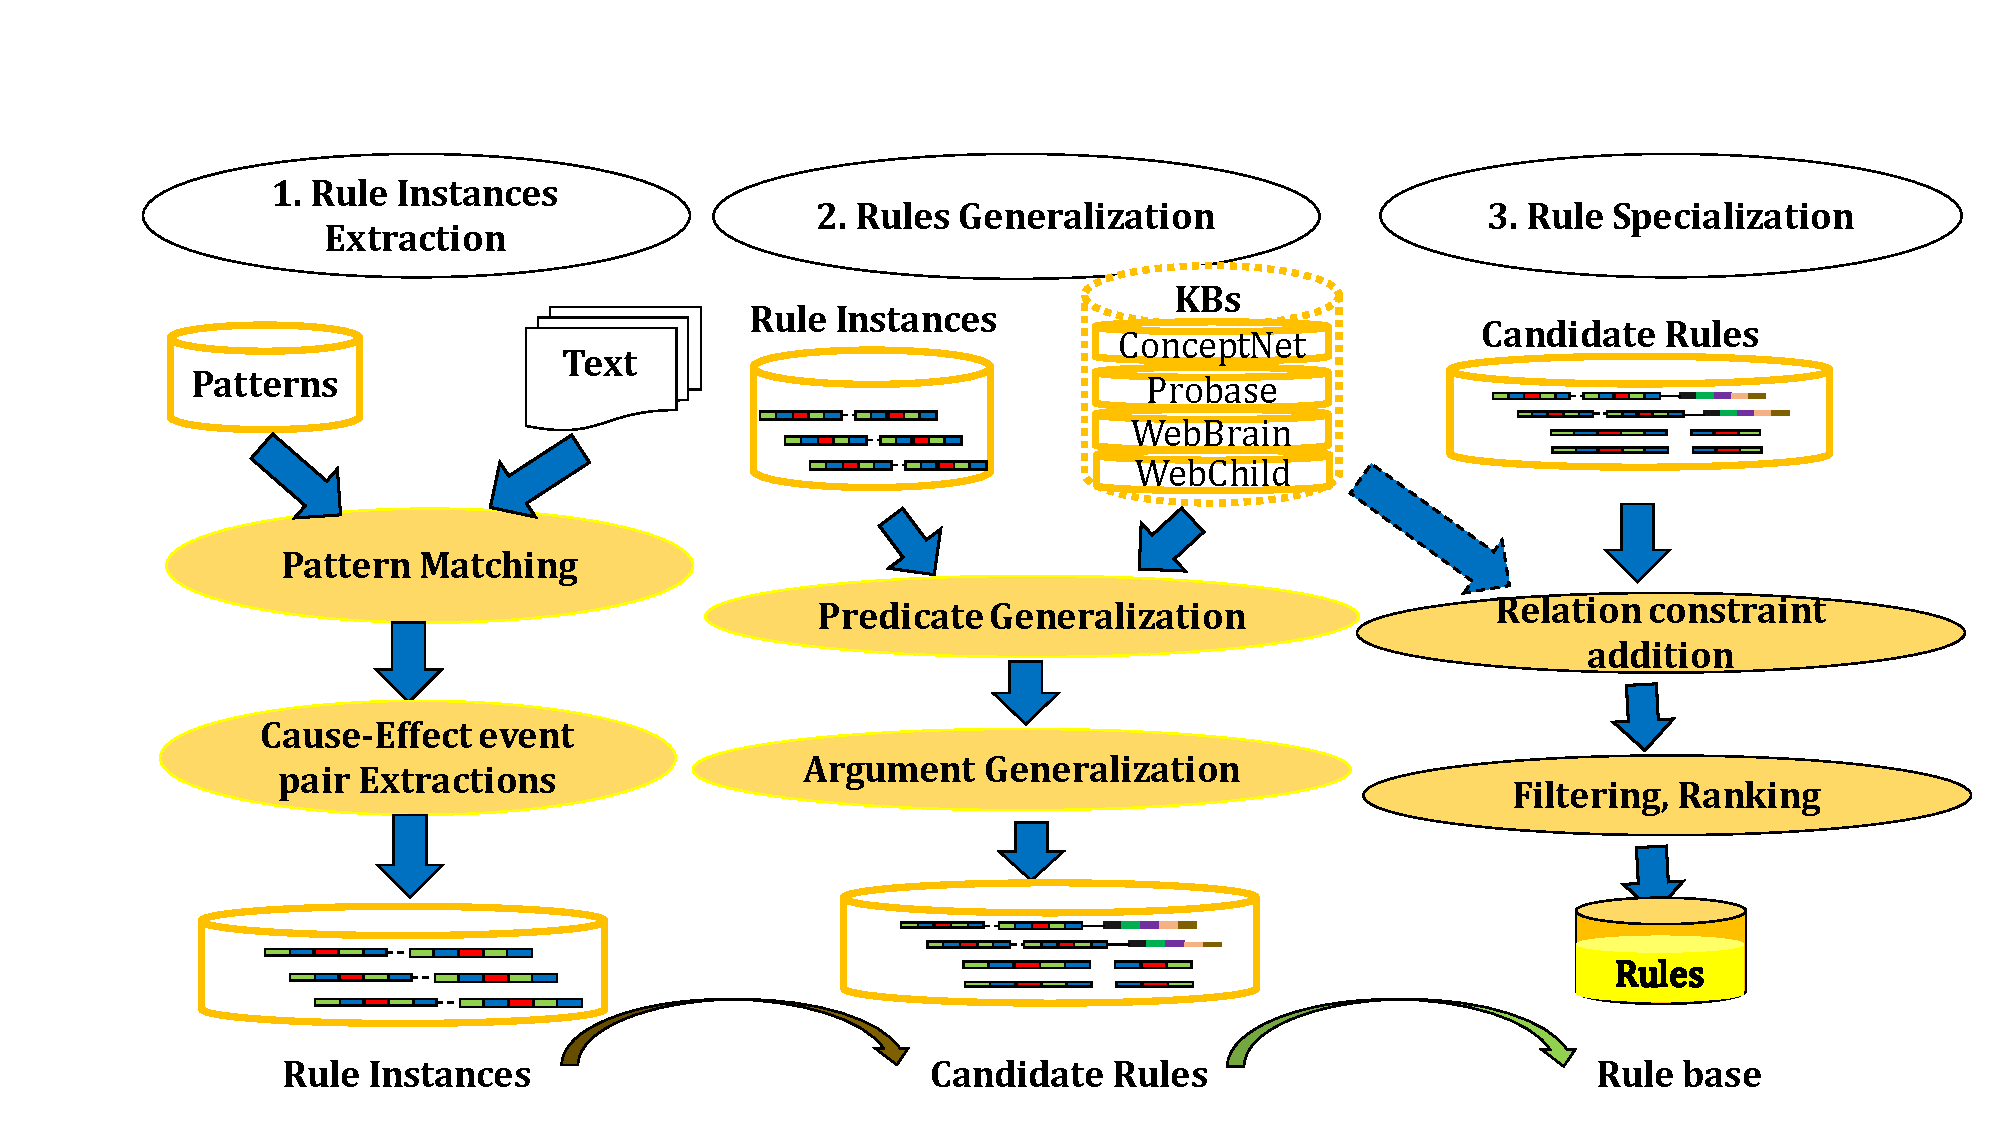
\includegraphics[width=\textwidth]{figures/overview}}
	\caption{Overview of our proposed framework.}
	\label{fig:overview}
\end{figure*}

%First of all, We need extract the cause and effect event span. Most of the approaches are based on elaborate patterns, We also follow the methods to extract the cause event span and effect span. for instance we '因为... 所以...' to catch the cause event span and effect event span. Alternatively, we can use a more sophisticated way to catch the causal relation such as \cite{b1} (Sendong Zhao 40), In this study, however, we focus more on the precision of extraction effect rather than the recall, also we think a more sophisticated method used on such already noisy text may lead to more errors.  

First of all, we extract the rule instances from liberal text shown in the graph\ref{fig:overview}'s left part. We firstly parse the sentences and use the elaborate causal patterns to match cause and effect span, then extract the event structure according to the dependency relations. After this step, We can get lots of rule instances each of which is composed by cause event and effect event.

Before, we further generalize the rule instances to candidate rules, we need a knowledge base, such a knowledge base should contain taxonomy which can hep ue do argument conceptualization and common sense which can help ue find relation constraints. We decide to construct such knowledge base contain common sense, since we find that most relations are common sense. besides our data is Chinese, only ConceptNet5\cite{speer2013conceptnet} satisfies our need, which has the Chinese resource. But the quantity is far from our expectation. So we decide to build a new one with fusion of many existing knowledge bases. For example, Probase\cite{wu2012probase} which is special for taxonomy, and ConceptNet5\cite{speer2013conceptnet}, WebBrain\cite{chen2016webbrain}, Webchild\cite{tandon2014webchild} which are specially aimed at  common sense.

Then, we would like to generalize these rule instances into candidate rules shown in the Figure \ref{fig:overview}'s middle part. This rule generalization component mainly contains two steps. The first step is predicate generalization and the second step is argument generalization. Predicate generalization is trying to normalize the similar predicates into the unified one. For example, "raise, rise, soar, increase, gain, enhance" have the same meaning, we need give a unified predicate to represent this group of predicates with the help of Cilin\footnote{ \url{ http://www.bigcilin.com/}}. Argument generalization step is trying to conceptualize the arguments in the rule instances which need to exploit the taxonomy in our built knowledge base. Since each candidate rule is derived by observing a cluster of similar rule instances, we need divide rule instances into several clusters. in each cluster, we generalize these rule instances to a candidate rule, and we will elaborate it in Section \ref{sec:approach}.         

Last, after rule generalization, we carry on rule specialization via adding relation constraints into the candidate rules. Since the candidate rules are general, we exploit our built knowledge base to specialize the candidate rules into real rules. The relations of each candidate rule is derived by finding the mutual relations existed in this candidate rule's supported rule instances cluster.

%So we need to specialize the candidate rules to real rules. we add some relation constraints to each candidate rule with the help of our built knowledge base. Since each rule has many supported rule instances, We just find the mutual relations existed in all rule instances. 

Above are main components of our proposed framework to mine causality knowledge.

\textbf{Contributions.}
To mine the causality knowledge, we propose a solution to mine the causality knowledge. And extensive experiment's results show that the mined rules are pretty good. Besides, we will release the some resource like the our built Chinese  knowledge base and rules.

The remainder of this paper is organized as follows. We define the necessary concepts and formulate the focal problem in Section \ref{sec:problem}. Our proposed approach are presented in Section \ref{sec:approach}. Section \ref{sec:experiment} reports the experimental observations followed by a brief review of related works in Section \ref{sec:related}. Section \ref{sec:conclusion} concludes the paper.
 
 
\section{PROBLEM DEFINITION}
\label{sec:problem}

In this section, we will formally state the focal problem to be solved.

%The list of major symbols and notations in this paper is summarized in the following table.

%\begin{table}[htbp]
%	\caption{Table of notations }
%	\begin{center}
%		\begin{tabular}{|c|l|}
%			\hline
%			\textbf{Notation}&\textbf{Definition}\\
%			\hline
%			rule instance & structured causality proposition pair\\
%			\hline
%			$E_{c_i}$ & the instances of $i-th$ concept \\
%			\hline
%			\multirow{2}{*}{rule}
%			& generalized rule instance with concept constraints \\
%			&and relation constraints \\
%			\hline
%		\end{tabular}
%		\label{tab1}
%	\end{center}
%\end{table}	

%our goal:
%	We try to make reasoning interpretable via symbol not neural network. 
% 
 \textbf{Problem Statement.} Mine the causality knowledge hidden in large amount of unstructured text and represent the causality knowledge with rule form (\ref{equ:rule_notation}).  